%\documentstyle[11pt,fullpage]{article}
%\setlength{\parindent}{0 in}
%\setlength{\parskip}{.1in}
%\setlength{\topmargin}{-0.5in}
%\setlength{\textheight}{8.5in}
%\begin{document}
\chapter{Directed Diffusion}
\label{chap:diffusion}

The directed diffusion module in ns has been ported from SCADDS group's implementation of directed diffusion at USC/ISI. There is an older version of diffusion in ns that was implemented several years back and has become relatively old and outdated. This older version can be found under directory diffusion. And the newer version of diffusion resides under \nsf{/diffusion3}. This chapter talks about the newer diffusion model in ns. The module and methods described here can be found under \nsf{tcl/lib/ns-diffusion.tcl, ns-lib.tcl} and all relevant C++ code can be found under \nsf{diffusion3}. Visit the SCADDS group webpage at \url{http://www.isi.edu/scadds} for details about their implementation.

\section{What is Directed Diffusion?}
Directed Diffusion is a method of data dissemination especially suitable in distributed sensing scenarios. It differs from IP method of communication. For IP ``nodes are identified by their end-points, and inter-node communication is layered on an end-to-end delivery service provided within the network''. Directed diffusion, on the other hand is data-centric. Data generated by sensor nodes are identified by their attribute-value pair. Sinks or nodes that request data send out ``interest''s into the network. Data generated by ``source'' nodes that match these interests, ``flow'' towards the sinks. Intermediate nodes are capable of caching and transforming data. For details on directed diffusion, see  
``Directed Diffusion: A Scalable and Robust Communication Paradigm for Sensor Networks'', authored by Chalermek Intanagonwiwat, Ramesh Govindan and Deborah Estrin that appeared in MobiCOM, August 2000, Boston, Massachusetts. This and other diffusion related papers can be viewed at \url{http://www.isi.edu/scadds/publications.html} under publications section.

\section{The diffusion model in ns}
\label{sec:diff_model}

The directed diffusion model consists of a core diffusion layer, a diffusion library provides an application programming interface for overlying diffusion applications and finally the application layer which includes both diffusion applications and filters. The core diffusion layer is used to receive/send out packets from/into the network. The library provides a interface for the overlying application classes for publishing/subscribing etc. These APIs have been described in details in a document called Network Routing API 8.0 and can be found at 
\url{http://www.isi.edu/scadds/publications.html} under APIs section. In the following paragraphs we are going to describe how the diffusion model looks like in \ns.


First we start with a brief description of the diffusion3 directory structure.
If the reader wishes to examine the C++ code related to NS Diffusion
that underpins the OTcl script commands, it may be found in
\nsf{ns/diffustion3}.�Here is a summary by subdirectory:
\begin{description}

\item[apps] contains sample source and sink applications like gear, ping and rmst.
\item[lib] has DiffusionRouting class definitions and definitions of diffusion application class. In addition there are sub-dirs called main and nr. main houses  misc diffusion utility code. nr includes attribute definition and the class NR which is an abstract factory for the API (so that either ISI or MIT implementations may derive from it.

\item[ns] contains ns wrappers for diffusion code.�These wrapper classes allow the core diffusion code and the diffusion API to be seamlessly incorporated into the NS class hierarchy. The DiffRoutingAgent is a wrapper for the Core Diffusion code, and DiffAppAgent is a wrapper for the DiffusionRouting (API) code.

\item[filter\_core] has the core diffusion agent.

\item[filters]  holds the different filters supported by diffusion implementation including two-phase-pull, one-phase-pull, gear, rmst, log, tag and srcrt (as of 10/03/03).
 
\end{description}

\begin{figure}[tb]
	\centerline{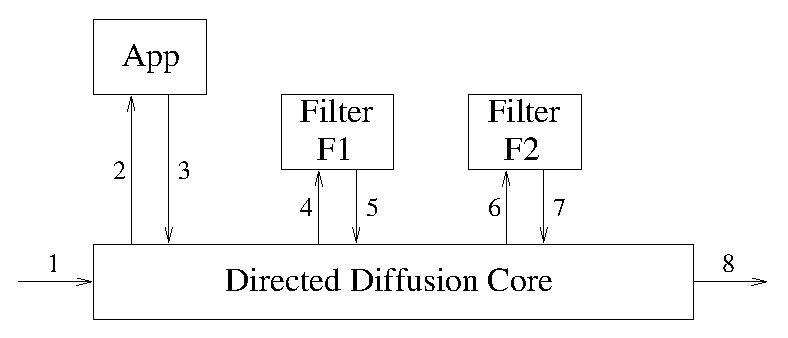
\includegraphics{filter}}
	\caption{Message flow in directed diffusion}
	\label{fig:filter}
\end{figure}


The above Figure~\ref{fig:filter} is from SCADDS' network routing API document available from their homepage (URL given earlier). The document describes attribute factories, matching rules for attributes, how applications interface with the core diffusion layer, and filter/timer APIs. All messages coming from/going out in the network is received at/sent out from the core diffusion layer. Messages can also come to core-diffusion layer from local applications and/or filters that might be connected to the node. The applications use the publish/subscribe/send interface to send interest and data messages to the network.

%\begin{figure}[tb]
%	\centerline{\includegraphics{directeddiffusion}
%	\caption{Schematic of a mobilenode supporting directed diffusion}
%	\label{fig:diffusion-node}
%\end{figure}

%% The above Figure~\ref{fig:diffusion-node} shows the internals of directed
%% diffusion implementation in \ns. 

The core diffusion agent and diffusion application agent are attached to two well-known ports defined in \nsf{/tcl/lib/ns-default.tcl}. Diffusion applications attached to the node call the underlying diffusion application agent for publishing/subscribing/sending data.

\section{Some mac issues for diffusion in ns}
In the shim layer that sits between diffusion and ns, (see diffusion3/ns dir for code implementing this layer) all diffusion packets are encapsulated within ns packets and are marked to be broadcasted. In previous versions all diffusion packets were marked to be broadcast in ns. This is now changed. Now all diffusion pkts in ns uses the diffusion next\_hop info thus allowing both broadcast and unicast.

So previously this only-brdcast feature supported for diffusion packets resulted in some problems at the mac layer. The mac-802.11 doesnot try to re-transmit a broadcast packet incase there is a collision and the packet is dropped. Coupled to this was the fact that mac-802.11 didn't do random selection of slots in the contention window before it transmitted a packet (a brdcast data or rts for unicast pkts). As a result there were a high number of collisions at the mac layer and a lot of packets were lost. This was fixed by adding random selection of slots before mac tx'ed a brdcast pkt (or a rts pkt).

However if we have a large and dense topology, there is a chance that two or more nodes may select the same slot in the mac contention window (the contention window size varies from 31 to 1023 for DSSS PHY MIB specifications). Thus now we need to add some extra jitter at the higher application layer. Diffusion has a provision to do this by compiling ns with the macro USE\_BROADCAST\_MAC. 
What this does is it in addition to delaying certain messages (to avoid collisions), when run with a BROADCAST MAC layer, diffusion will use a different set of values for delays and jitters. These different delay/jitter values are defined under diffusion3/lib/main/config.hh. Since this might increase the latency 
you might want to fine-tune the delay values by hand. 

\section{APIs for using filters in diffusion}
\label{sec:diff_filter}

As described earlier (see figure~\ref{fig:filter}), filters can be attached to a diffusion node for various reasons. There can be basic diffusion filters providing two-phase-pull (GradientFilter) and one-phase-pull (OnePhasePullFilter) diffusion routing algorithms. There is the GeoRoutingFilter or gear that provides a certain location (co-ordinate) based routing algorithm. There is also other filters for RMST routing algorithm (RmstFilter), logging (LogFilter), source routing (SourceRouteFilter) and tagging (TagFilter). See Commands at a glance section for details on APIs for adding filters to a diffusion node.


\section{Ping: an example diffusion application implementation}
\label{sec:ping_app}

There is a ping application implemented under diffusion3/apps/ping subdir. The application consists of a ping sender and receiver. The receiver requests for data by sending out ``interest''s in the network. The interests get diffused through the network. The ping-sender on receiving matching interests, sends out data. 


\subsection{Ping Application as implemented in C++}
\label{sec:ping_cpp}

The ping-sender and -receiver classes, namely PingSenderApp and PingReceiverApp both derive from DiffApp, the parent class for all diffusion based applications. See diffusion3/lib/diffapp\{.cc,.hh\} for detailed implementation of the DiffApp class.

The ping-sender uses MySenderReceive object that handles all callbacks for it. Also the ping-sender defines two functions setupSubscription() and setupPublication(). 
The first function creates interest attributes that matches with data attributes it (the sender) has to offer. Next it calls the dr-library function subscribe(). The subscription is used by the ping-sender to create an internal state against which attributes for interests received from the network are matched against. Incase of a match, the matching data is sent outinto the network. Function setupPublication() create attributes for the data it has to offer and calls the library function publish() which inturn returns a publish handle. The ping-sender uses this handle to periodically send out data which is forwarded by the gradient to core-diffusion to be sent out into the network only if it finds a matching interest.

The ping-receiver object uses a similar callback object called MyReceiverReceive. And it defines a function setupSubscription() that creates attributes for the interest the receiver will be sending. Next it calls the dr library supported subscribe() which sends the interest out into the network. The recv() function is used to recv matching data and the receiver then calculates the latency for each data packet received from the ping-sender.
The ping sender can be found under ping\_sender{.cc,.h}. And the ping\_receiver is implemented under ping\_receiver{.cc,.h}. Some common defines and attribute factories for data/interest attributes are defined in ping.hh and ping\_common.cc.

\subsection{Tcl APIs for the ping application}
\label{sec:ping_tcl}

An example script for the ping application is under \nsf{tcl/ex/diffusion3/simple-diffusion.tcl}. The example scenario consists of 3 nodes of which one is a ping-sender and another is a ping-receiver. The source and sink nodes are far away from one another and communicate only through a third node. The option adhocRouting is defined as Directed\_Diffusion. This enables a core-diffusion agent to be created during the time of node creation. Also it creates a diffusionApplication agent if one is not present already. The option diffusionFilter needs to be provided at the time of node configuration that defines the one or more filters that would be added to the node. There is also an option for specifying stopTime which is the time the simulation ends. At this time there is a callback to a function that prints out all statistical data into /tmp/diffusion-*.out.

Node configuration is done as follows:
\begin{program}
$ns_ node-config -adhocRouting $opt(adhocRouting) \
                 -llType $opt(ll) \
                 -macType $opt(mac) \
                 ....
                 -diffusionFilter $opt(filters) \
                 -stopTime $opt(prestop) \
                 -agentTrace ON \
                 ....
\end{program}

The ping sender application is created in the following way:
\begin{program}
set src_(0) [new Application/DiffApp/PingSender]
$ns_ attach-diffapp $node_(0) $src_(0)
$ns_ at 0.123 "$src_(0) publish"

\end{program}

The first line creates a ping-sender object. Simulator class method attach-diffapp basically attaches the application to the underlying diffusionApplication agent for that given node.
The command \code{publish} essentially ``starts'' the sender application.

Similarly the ping sink is created as follows:
\begin{program}
#Diffusion sink application
set snk_(0) [new Application/DiffApp/PingReceiver]
$ns_ attach-diffapp $node_(2) $snk_(0)
$ns_ at 1.456 "$snk_(0) subscribe"
\end{program}

The command \code{subscribe} starts the ping-receiver application.

Thus in order to create your own application, you need to :
\begin{description}
\item[1.] define attribute-factories and attributes for application interest/data.
\item[2.] create the application class (using dr-library APIs)
\item[3.] add tcl commands to start the application
\end{description}

See \nsf{tcl/lib/ns-lib.tcl, ns-diffusion.tcl} for implementations of OTcl hooks for directed diffusion. Alo see chapter on Mobility in this manual for details on mobility model and wireless simulations in \ns.


\section{Changes required to add yr diffusion application to ns}
Let's say you have an application (it might even be a certain filter, which also is by class hierarchy, a diffusion application and it would derive from class DiffApp) that runs on the test-bed version. Now you want to run diffusion on ns and so want to use yr application in the ns context. The few lines describe the changes/additions you need to make for yr diffusion application to work in ns environment.

We will consider onePhasePullFilter object (under diffusion3/filters/misc/log.*) as an example. As a first step you need to create a split object out of the application class object, presumably defined as a pure c++ object. A split object is one that is created by the user in the interpretor (in OTcl space) and which is also has a shadow object in the compiled hierarchy (in c++ space). In ns, a split object is derived from class TclClass as shown below:

\begin{program}
#ifdef NS_DIFFUSION
static class LogFilterClass : public TclClass {
public:
  LogFilterClass() : TclClass("Application/DiffApp/LogFilter") {}
  TclObject * create(int argc, const char*const* argv) {
    return(new LogFilter());
  }
} class_log_filter;
#endif //DIFFUSION
\end{program}

Note that all filter objects specifically have a handle to the DiffAppAgent (the diffusion routing object) passed in the constructor call. Filter objects get created from function create-diffusionApp-agent {diffFilters} defined in ns-diffusion.tcl. Users need not specifically call the OTcl function create-diffusionApp-agent as it is called during node creation based on the node-configuration parameters. See how filters are defined in node-config under commands at a glance section. 
However application objects which are not filter objects (like ping\_sender, push\_receiver etc) are created by users directly from user scripts. And in that case the handle to DiffAppAgent is passed using \code{$ns attach-diffapp $node $app}
where the application \code{$app} is attached to the node object \code{$node}.

So for the reasons explained above the constructors are different in non NS\_DIFFUSION context as shown below.  

\begin{program}

#ifdef NS_DIFFUSION
LogFilter::LogFilter()
#else
LogFilter::LogFilter(int argc, char **argv)
#endif // NS_DIFFUSION
{
  // Create Diffusion Routing class
#ifndef NS_DIFFUSION
  parseCommandLine(argc, argv);
  dr_ = NR::createNR(diffusion_port_);
#endif // !NS_DIFFUSION

  filter_callback_ = new LogFilterReceive(this);

#ifndef NS_DIFFUSION
  // Set up the filter
  filter_handle_ = setupFilter();
  ...
  ...
#endif // !NS_DIFFUSION
}

\end{program}

Next you need to add the c++ function command(..) that allows execution of tcl commands through the compiled shadow object. For example the otcl command \code{start} is used to start a filter application as follows \code{$app start}. While commands \code{publish} and \code{subscribe} are used to start sender and receiver applications respectively. The command function is added, again with the NS\_DIFFUSION scope using ifdef statements, as follows:

\begin{program}
#ifdef NS_DIFFUSION
int LogFilter::command(int argc, const char*const* argv) {
  if (argc == 2) {
    if (strcmp(argv[1], "start") == 0) {
      run();
      return TCL_OK;
    }
  }
  return DiffApp::command(argc, argv);
}
#endif // NS_DIFFUSION
\end{program}
 
Note how the parent class command function is invoked incase the command string is not found. Look into lib/diffapp.* to see all otcl commands supported for the DiffApp class.

Once these changes made to your c++ code, you would also need to write a tcl script (see the section on test-suite for example tcl scripts) that uses your diffusion application using the right tcl APIs.


\section{Test-suites for diffusion}
\label{sec:test_diff}

we start with a simple testcase of 3 nodes with 1 ping source and 1 ping sender. There are other tests for 2 phase-pull(2pp), 1 phase-pull(1pp), push and gear (with 2pp and push) scenarios. In future we plan to extend the test-suite for testing different components/functionalities of directed diffusion. All diffusion3 related test cases can be found under \nsf{tcl/test/test-suite-diffusion3.tcl}.


\section{Commands at a glance}
\label{sec:directeddiffusion}

Following is a list of commands used for diffusion related simulation in ns. 

\begin{program}
$ns_ node-config -adhocRouting $opt(adhocRouting) 
	         -llType $opt(ll)
                  ...
	         -diffusionFilter $opt(filters)
                 -stopTime $(pre-stop)
                  ...
where,
value of opt(adhocRouting) is set to Directed_Diffusion
This command is used to enable directed diffusion in wireless nodes.

value of opt(filters) can be a list of filters that is required to be attached to diffusion nodes each separated by a forward-slash like GradientFilter/GeoRoutingFilter/TagFilter or maybe GradientFilter/TagFilter etc.
This command allows adding filter objects to diffusion-enabled nodes.

value of opt(pre-stop) is usually the time simulation stops when all statistical data is dumped into a file.
This command allows dumping of statistical data into an output file after running a diffusion simulation.
\end{program}


\begin{flushleft}
\code{ set src [new Application/DiffApp/PingSender]}\\
This command is used to create ping-sender application.

\code{set snk [new Application/DiffApp/PingReceiver]}\\
This command is used to create ping-receiver application.

\code{ set src [new Application/DiffApp/PushSender]}\\
This command is used to create push-sender application.

\code{set snk [new Application/DiffApp/PushReceiver]}\\
This command is used to create push-receiver application.

\code{ set src [new Application/DiffApp/GearSenderApp]}\\
This command is used to create gear-sender application.

\code{set snk [new Application/DiffApp/GearReceiverApp]}\\
This command is used to create gear-receiver application.

\code{$gearApp push-pull-options <push/pull> <point/region> <co-ordinatesX1> <X2> <Y1> <Y2>}
This command defines the type of routing algorithm gear is using. Incase the second option is defined as region, all four co-ordinates should be defined. While if point is chosen, only X1 and Y1 maybe defined.

\code{$ns_ attach-diffapp $node_ $src_}\\
where the diffusion application \code{$src_} gets attached to the given \code{$node_}.

\code{$src_(0) publish}\\
Command to start a ping source (sender).

\code{$snk_(0) subscribe}\\
Command to start a ping sink (receiver).

\end{flushleft}
%\end{document}
\endinput
